\section{Introduction}
According to research done by Nash Networks \cite{choudhary} in 2008, 70\% of e-mail is estimated to be spam. Furthermore, up to employees can spend up to 16 minutes per week on spam management. While this may seem like a small number, an organization with 50 employees can waste more than \$20,000 per year in lost employee time simply due to spam management. Thus, the costs of spam are  high for most large companies, so there is a demand for more effective methods of spam filtering. We have attempted to analyze the relative performance of three types of machine learning-based spam filtering techniques: support-vector machines (SVM), decision trees, and AdaBoost.

To accurately assess the performance of these machine learning algorithms, we must also address the challenge of good feature selection. Feature selection is the process of selecting appropriate elements of a data set to measure in order to construct a model. Too many features can result in what is called "overfitting," where a machine learning algorithm will be able to operate perfectly on its training dataset, but its learned knowledge is useless for any other dataset. Too few features results in an algorithm that cannot accurately categorize inputs. For this project, our features consisted of words in various emails. The block diagram in Figure~\ref{fig:featureSelection} illustrates the process of feature extraction/selection. 



\begin{figure}[h]
    \centering
    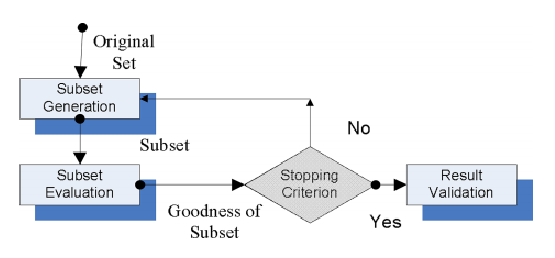
\includegraphics[width=0.5\textwidth]{featureSelection}
    \caption{Feature Selection}
    \label{fig:featureSelection}
\end{figure}
